\documentclass{beamer}

\usepackage{amsfonts}
\usepackage{amsmath}
\usepackage{longtable}
\usepackage{csquotes}
\usepackage{standalone}

\usepackage{graphicx}
\graphicspath{{../pictures/}}

\usepackage{tikz}
\usetikzlibrary{shapes, calc, arrows, decorations.markings,
  decorations.pathmorphing, decorations, patterns, chains, snakes,
  backgrounds, positioning, fit, petri}
\newcommand{\inputpicture}[1]{\input{../drawings/#1}}

\usepackage{listings}
\lstset{language=C, basicstyle=\ttfamily, breaklines=true, keepspaces=true,
  keywordstyle=\color{blue}}

\usepackage{bytefield}

\usefonttheme{professionalfonts}
\usefonttheme{serif}
\usepackage{fontspec}
\setromanfont{CMU Serif}
\setsansfont{CMU Sans Serif}
\setmonofont{CMU Typewriter Text}

\usepackage{hyperref}
\hypersetup{colorlinks=true, linkcolor=black, filecolor=black, citecolor=black,
  urlcolor=blue , pdfauthor=Evgenii Iuliugin <yulyugin@gmail.com>,
  pdftitle=Fundamentals of Full-Platform Simulation}

\usepackage{underscore}
\usepackage{amsthm}

\subtitle{Fundamentals of Full-Platform Simulation}
\subject{Lecture}
\date{\today}

\author[Evgenii Iuliugin]{
  Evgenii Iuliugin \small{\href{mailto:yulyugin@gmail.com}{yulyugin@gmail.com}}}
\typeout{Copyright 2021 Evgenii Iuliugin}

\usetheme{Berlin}
\setbeamertemplate{navigation symbols}{}

\newcommand{\finalslide}{
    {\huge{Thank you!}\par}

    \vfill
    Slides and material are available at
    \url{https://github.com/yulyugin/sim-lectures}
    \vfill

    \tiny{\textit{Note}: All trademarks are the property of their respective
        owners.
        The presented point of view reflects the personal opinion of the author.

        %All the materials are licensed under the Creative Commons
        %Attribution-NonCommercial-ShareAlike 4.0 Worldwide. To view a copy of
        %this license, visit
        %\url{http://creativecommons.org/licenses/by-nc-sa/4.0/}.
    }
}

\title{Cycle-Accurate Simulation}

\begin{document}

\startslides

\begin{frame}{On the Previous Lecture:}
\begin{itemize}
\item Simulation of architectural state:
  \begin{itemize}
  \item register file --- fields, banks,
  \item lazy calculations,
  \item large arrays --- memory, disk\dots
  \end{itemize}
\item Functional full-platform simulation:
  \begin{itemize}
  \item Executing devices: interpreter, JIT, direct execution.
  \item Non-executing devices: discrete event simulation.
  \end{itemize}
\end{itemize}
\end{frame}

\begin{frame}{Questions}
\begin{itemize}
\item How many bits are in a machine word?\pause
\item What is better MMIO or PIO?\pause
\item Can an architecture be neither big-endian nor little-endian?\pause
\end{itemize}
\end{frame}

\section{Cycle-Accurate Models}

\begin{frame}{Simulated System}
\centering
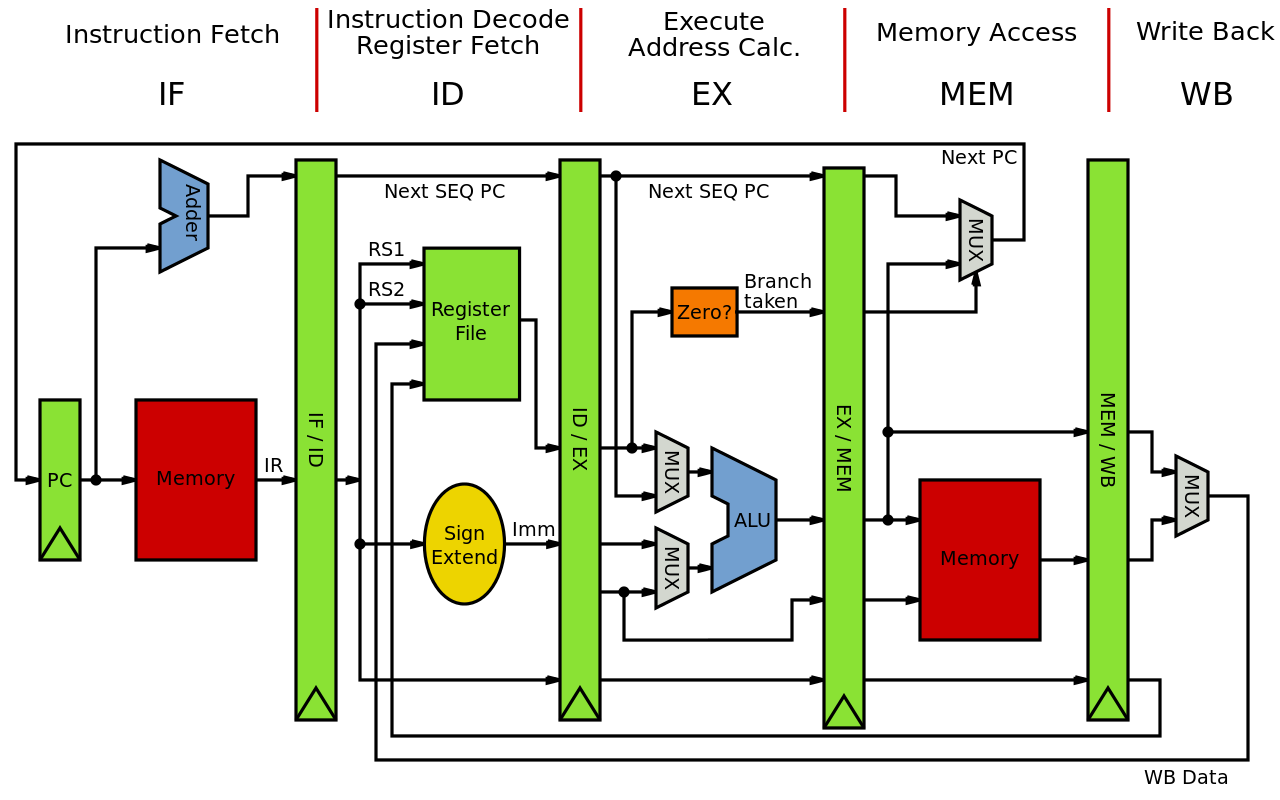
\includegraphics[width=\textwidth]{./mips-arch}

\tiny{\url{http://commons.wikimedia.org/wiki/File:MIPS_Architecture_(Pipelined).svg}}
\end{frame}

\begin{frame}{Problems}
\begin{itemize}
\item Functional models --- not applicable (too approximate).
\item DES --- applicable but not representative abstraction.
\end{itemize}
\vfill
\centering
\inputpicture{des-long}
\end{frame}

\begin{frame}{Properties}
\centering
\inputpicture{features}
\end{frame}

\begin{frame}{Problems}
\begin{itemize}
\item The same operation may have different duration for different nodes.
\item How to check readiness for <<slow>> nodes?
\item Results should not be available before the next cycle.
\end{itemize}
\end{frame}

\section{Functions And Ports}

\begin{frame}{Solution --- Functions And Ports}
Split:
\begin{itemize}
\item Node functions.
\item Time to complete the functions.
\item Internal state of node.
\end{itemize}
\end{frame}

\begin{frame}{Function}
The results is ready <<immediatelly>> if input data is available.
\vfill
\centering
\inputpicture{pure-function}
\end{frame}

\begin{frame}{Port}
Port is a queue with fixed delay.
\vfill
\centering
\inputpicture{delay-line}
\end{frame}

\begin{frame}{Connection Rules}
\begin{itemize}
\item Functions cannot be connected directly to each other.
\item Simulation phases alternate:
  \begin{enumerate}
  \item Function simulation;
  \item Result transfer simulation.
  \end{enumerate}
\end{itemize}
\end{frame}

\begin{frame}{Simulation: Phase 1 --- Functions}
\centering
\inputpicture{cycle-phase1}
\end{frame}

\begin{frame}{Simulation: Phase 2 --- Ports}
\centering
\inputpicture{cycle-phase2}
\end{frame}

\section{Implementation Details}

\begin{frame}{Data Readiness}
\centering
\inputpicture{valid}
\end{frame}

\begin{frame}{State Of a Functional Element}
\centering
\inputpicture{state-storing}
\end{frame}

\begin{frame}{Node Composition}
\centering
\inputpicture{ports-compose}
\end{frame}

\begin{frame}{Approximate Timing}
\centering
\inputpicture{functional-cycle-accurate-connection}
\end{frame}

\begin{frame}{Full Speed Ahead}
\centering
\inputpicture{full-speed-ahead}
\end{frame}

\section*{Conclusions}

\begin{frame}{Conclusions}
\begin{itemize}
\item Cycle-accurate simulation.
\item Functions and ports.
\item Approximate timing.
\item Full speed ahead.
\end{itemize}
\end{frame}

\begin{frame}[allowframebreaks]{Bibliography}
\begin{thebibliography}{99}
\bibitem{} \textit{John L. Hennessy, David A. Patterson},
  Computer Architecture: A Quantitative Approach.
\bibitem{} \textit{M.~Pellauer, M.~Vijayaraghavan, M.~Adler, Arvind, J.~Emer},
  A-Ports: an efficient abstraction for cycle-accurate performance models on
  FPGAs.
\bibitem{} \textit{J.~Emer, P.~Ahuja, E.~Borch, A.~Klauser, C.~Luk,
  S~.Manne, S.~Mukherjee, H.~Patil, S~.Wallace, N.~Binkert, R.~Espasa, T.~Juan},
  Asim: A Performance Model Framework.
\bibitem{} \textit{A.~Sandberg, N.~Nikoleris, T.~E.~Carlson, E.~Hagersten,
  S.~Kaxiras and D.~Black-Schaffer}, Full Speed Ahead: Detailed Architectural
  Simulation at Near-Native Speed.
\bibitem{} \textit{B.~Borgstr\"{o}m, A.~Sembrant, D.~Black-Schaffer}, Adaptive
  cache warming for faster simulations.
\end{thebibliography}
\end{frame}

\begin{frame}{On the Next Lecture:}
Hardware assisted virtualization:
\begin{itemize}
\item Formal requirements.
\item Contemporary architectures.
\item Address translation.
\item Devices.
\end{itemize}
\end{frame}

\finalslide

\end{document}
